%% summary.tex
%% Copyright 2022 skyleaworlder
%
% This work may be distributed and/or modified under the
% conditions of the LaTeX Project Public License, either version 1.3
% of this license or (at your option) any later version.
% The latest version of this license is in
%   http://www.latex-project.org/lppl.txt
% and version 1.3 or later is part of all distributions of LaTeX
% version 2003/12/01 or later.
%
% This work has the LPPL maintenance status "maintained".
%
% This Current Maintainer of this work is skyleaworlder.
%
% This work consists of all the *.tex and *.sty files in
%   https://github.com/TJ-CSCCG/Tongji-Beamer
\section{总结与反思}
\begin{frame}{里程碑1小组工作亮点}
    \begin{itemize}
        \item 本次里程碑1开发过程中,我们小组充分阅读分析了甲方的SRS报告,进行功能抽取和接口设计,随后再基于接口进行开发的方式,以接口为单位分配开发任务到组员个人进行开发,总体工作分配非常顺畅,组员整体参与度和开发效率都达到了一个非常高的水平。
        \item 在项目开发初期,我们使用Tornado框架搭建了一套完整可用的企业级Web应用后端架构,通过仔细的模块设计与代码实现,成功做到了组员开发的接口模块之间的完全解耦合,使得组员能够各自顺畅地在功能分支上进行开发,仅需要改动自己负责的接口实现模块文件,而不需要改动其他组员的代码,这样的开发方式极大地提高了开发效率,也使得项目开发过程中在分支提交和合并的时候基本没有遇到任何冲突问题,极大提升了开发效率。
    \end{itemize}
\end{frame}

\begin{frame}{技术债}
    \begin{itemize}
        \item 当前我们项目的前端页面参考了开源项目sd webui,集成了gradio框架用以生成绘图界面UI,这使得我们的功能页面之间的前端技术栈过于复杂,不利于后期的功能扩展和维护。在之后的迭代中,我们考虑充分深入仔细地进一步研究sd webui的实现原理,使用H5+CSS+Vue.js进行页面重构,从而使得项目的前端技术栈更加简洁,易于维护。
        \item 当前限于服务端GPU的硬件运算能力,网站并不能很好地支持多用户并发,比如如果多个用户同时生成图片,可能会出现GPU算力不够的情况。因此,之后的里程碑中,我们考虑使用华为云的GPU算力服务,使得网站能够支持更多用户的并发访问。
        \item 本次迭代中仅实现了SRS大功能模块中的部分基础功能,软件系统的体量依然需要继续进行扩展,比如增加管理员机制、完善模型文件管理功能、完善用户搜索Prompt、用户展示生成图片与所用Prompt等等交互逻辑等一系列内容。
    \end{itemize}
\end{frame}

\begin{frame}{技术债}
    \begin{itemize}
        \item 当前第一次迭代过程中,我们小组并没有在开发环境中搭建测试相关的自动化流程架构,所有的接口我们都是通过Apifox工具,手动填入用例后发送,然后观察后端行为和返回结果来验证接口实现正确性。并且,由于没有测试门禁规则,导致开发初期组员偶尔会错误地提交自己对于关键配置文件(如MySQL和Redis的账号、端口和密码配置)的代码更改,并且将更改错误地合并到主分支。这导致其它组员将更改拉取到本地后,需要再手动将配置进行改回。之后的开发流程中,可以通过部署测试门禁等方式,进一步提升项目开发的规范性和开发效率。
    \end{itemize}
\end{frame}

\begin{frame}{项目组织情况}
    \begin{itemize}
        \item 里程碑1开发过程中,我们小组严格贯彻落实开发章程,每个礼拜组织组会和集中开发,每个人都积极参与讨论、构思和代码实现工作,能够按时按质完成自己的开发任务,开发效率非常高。
        \item 从下图中,可以看到组员们开发时忙碌而有条不紊的身影:
    \end{itemize}
\end{frame}

\begin{frame}{项目组织情况}
    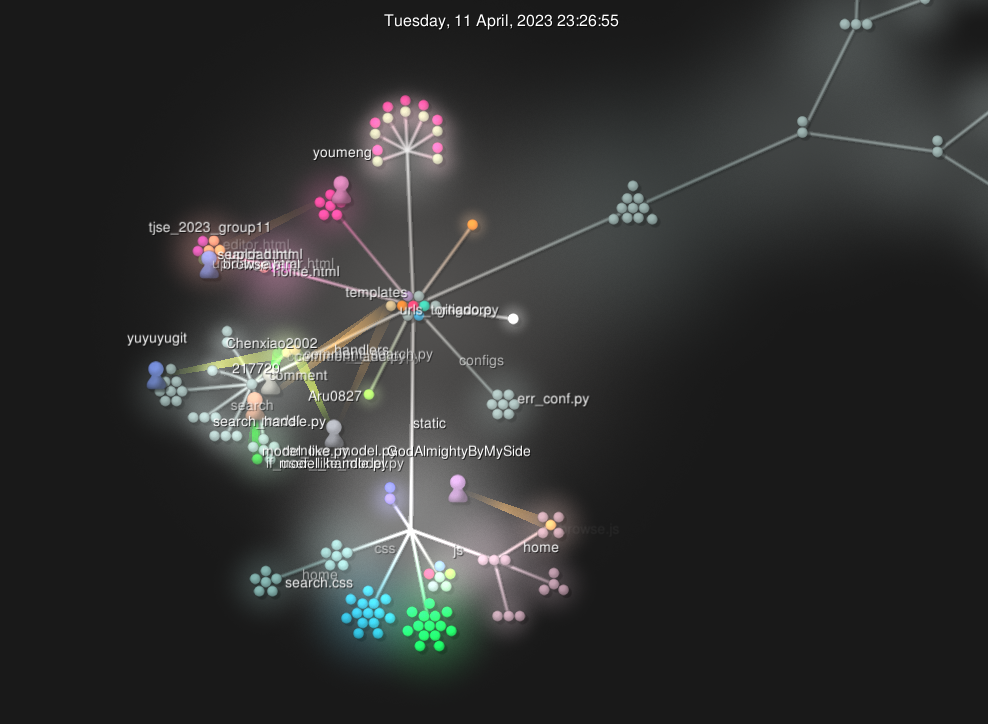
\includegraphics[width=1\textwidth]{contents/figure/commits.png}
\end{frame}

\begin{frame}{项目进度规划}
    \begin{itemize}
        \item 里程碑1:第7周到第9周,初步完成项目框架搭建
        \item 里程碑2:第10周到12周,在里程碑1的基础上,对页面进行重构,增加更多功能
        \item 里程碑3:第13周到15周,实现一个基本满足需求项目书要求的完整项目
        \item 里程碑4:第15周到17周,进行全面总体的功能测试,修改潜在bug并完善细节
    \end{itemize}
\end{frame}